% ch06: 原文 GLDraft_D.tex 行 1152–1382；§4.1–4.2
% 只译散文（标题、正文、图题、脚注）；公式、\label、\ref、\eqref、\cite、图文件名保持不变。

\section{Hecke、't Hooft 与 Wilson 算符}\label{wtw}

\subsection{线算符}

在几何朗兰兹纲领的通常表述中 \cite{BD}，主要研究对象包括作用在 $A$-膜范畴上的 Hecke 函子，以及这些 Hecke 函子的“本征膜”。\zy{“本征膜”（eigenbrane）是 Beilinson--Drinfeld 的“Hecke 本征层”（Hecke eigensheaf）在膜语言中的说法：Hecke 函子作用在它上面，只相当于再张量上某个固定的向量空间。参见 \cite{BD}；规范场论图像中的对应讨论见 \cite{KW}。}

在规范场论的图像中 \cite{KW}，Hecke 函子用 't Hooft 线算符来解释。电–磁对偶把 't Hooft 线算符映为 Wilson 线算符，由此得到关于几何朗兰兹对偶的一些通常陈述。

一般地，在二维拓扑场论中，线算符给出作用在边界条件范畴上的函子：这是因为，与以膜 $\B$ 标记的边界平行放置的线算符 $T$ 可以移动到该边界上，从而形成复合边界条件 $T\B$（图 \ref{example1}(a)）。这里我们假定二维流形与线算符（更确切地说，是承载它的那个一维流形）都带定向，并且线算符的定向与它所作用的边界的定向一致。同一幅图也点明了线算符的伴随（adjoint）这一概念。线算符的伴随 $T'$ 就是取相反定向的同一个线算符。在图 \ref{example1}(a) 中，我们可以把线算符 $T$ 移到图的右侧。此时它的定向与右侧边界的定向相反，于是给出对偶线算符 $T'$ 在定义右侧边界条件的膜 $\B'$ 上的作用。因此，对任意 $\B,\B'$，都有 $\Hom(\B',T\B)=\Hom(T'\B',\B)$。（有些线算符满足 $T$ 同构于 $T'$；它们的支撑集可以是不带定向的一维流形。）

这些陈述在任何二维拓扑场论中都成立。我们的实际应用涉及一个四维理论，它带有两个额外维度，二者合起来构成一个黎曼曲面 $C$。虽然可以考虑支撑集为四维流形 $\Sigma\times C$ 中任意曲线 $\gamma$ 的 't Hooft 算符（或对偶的 Wilson 算符），但我们只考虑 $\gamma=\ell\times p$ 这一特殊情形，其中 $p$ 是 $C$ 中的一点，$\ell$ 是 $\Sigma$ 中的一条曲线。因此，我们的线算符部分地由 $p$ 的选择来确定。此外，在应用到几何朗兰兹纲领时，'t Hooft 算符由 $G^\vee$（等价地，$G^\vee_\C$）的一个有限维不可约表示 $R$ 来标记。若要指明这一数据，我们把该 't Hooft 算符记作 $T_{R,p}$。类似地，依赖于表示 $R$ 与点 $p$ 的对偶 Wilson 算符将记作 $W_{R,p}$。


 \begin{figure}
 \begin{center}
   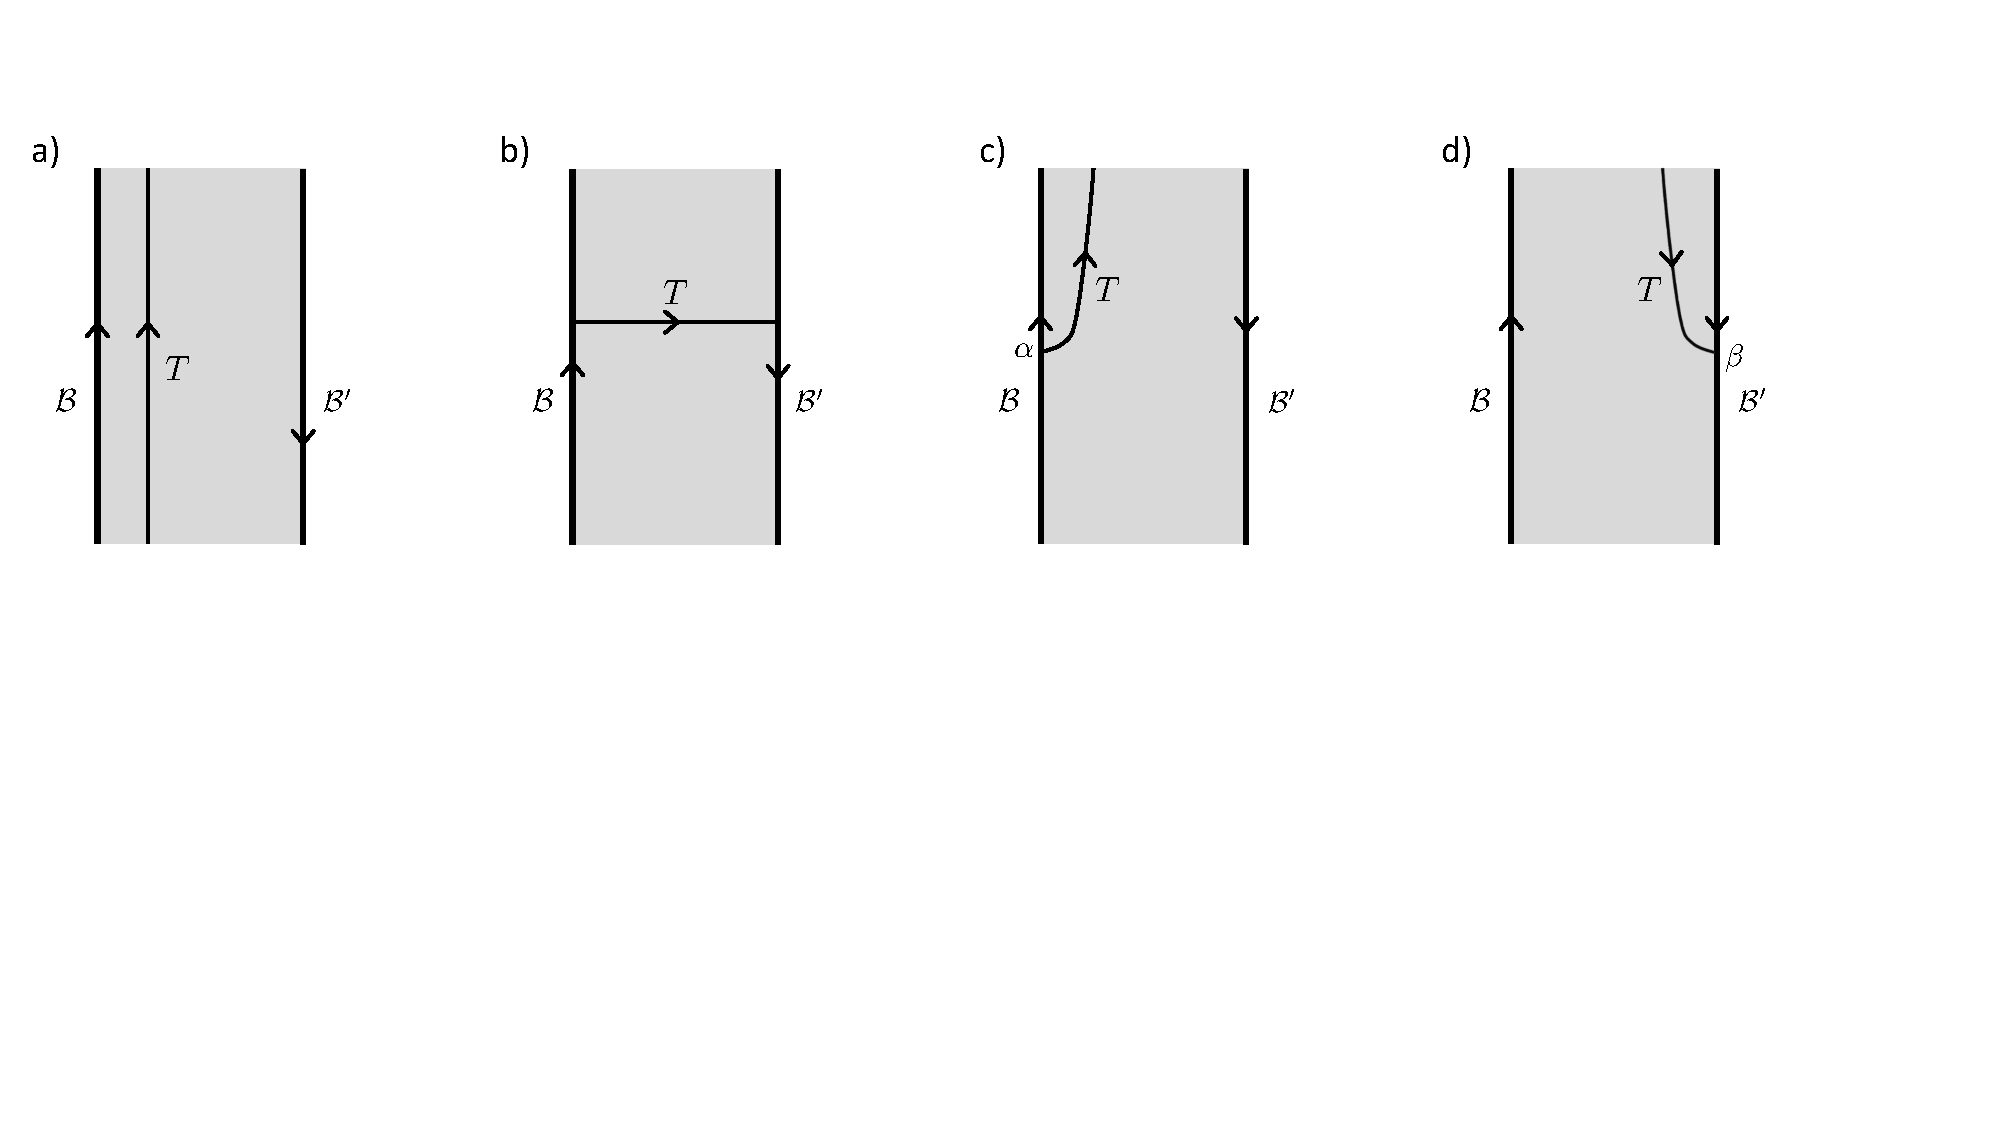
\includegraphics[width=6.2in]{Example1.pdf}
 \end{center}
\caption{\small (a) 与条带左边界平行、且定向与之相容的线算符 $T$。把 $T$ 向左移动，它把标记为 $\B$ 的边界条件映为复合边界条件 $T\B$。这就是把线算符视为膜或边界条件范畴上的函子，正如几何朗兰兹纲领的通常表述那样。(b) 在几何朗兰兹对偶的解析进路中，同一个线算符 $T$ 水平横穿条带，并在端点处带有某些额外数据，于是成为作用在物理态上的算符。(c) 与 (d) 这些图意在阐明 (b) 中左右两端所需的额外数据。在左端点有一个元素 $\alpha\in \Hom(\B,T\B )$，在右端点有一个元素 $\beta\in\Hom(T\B',\B')$。 \label{example1}}
\end{figure} 


 \begin{figure}
 \begin{center}
   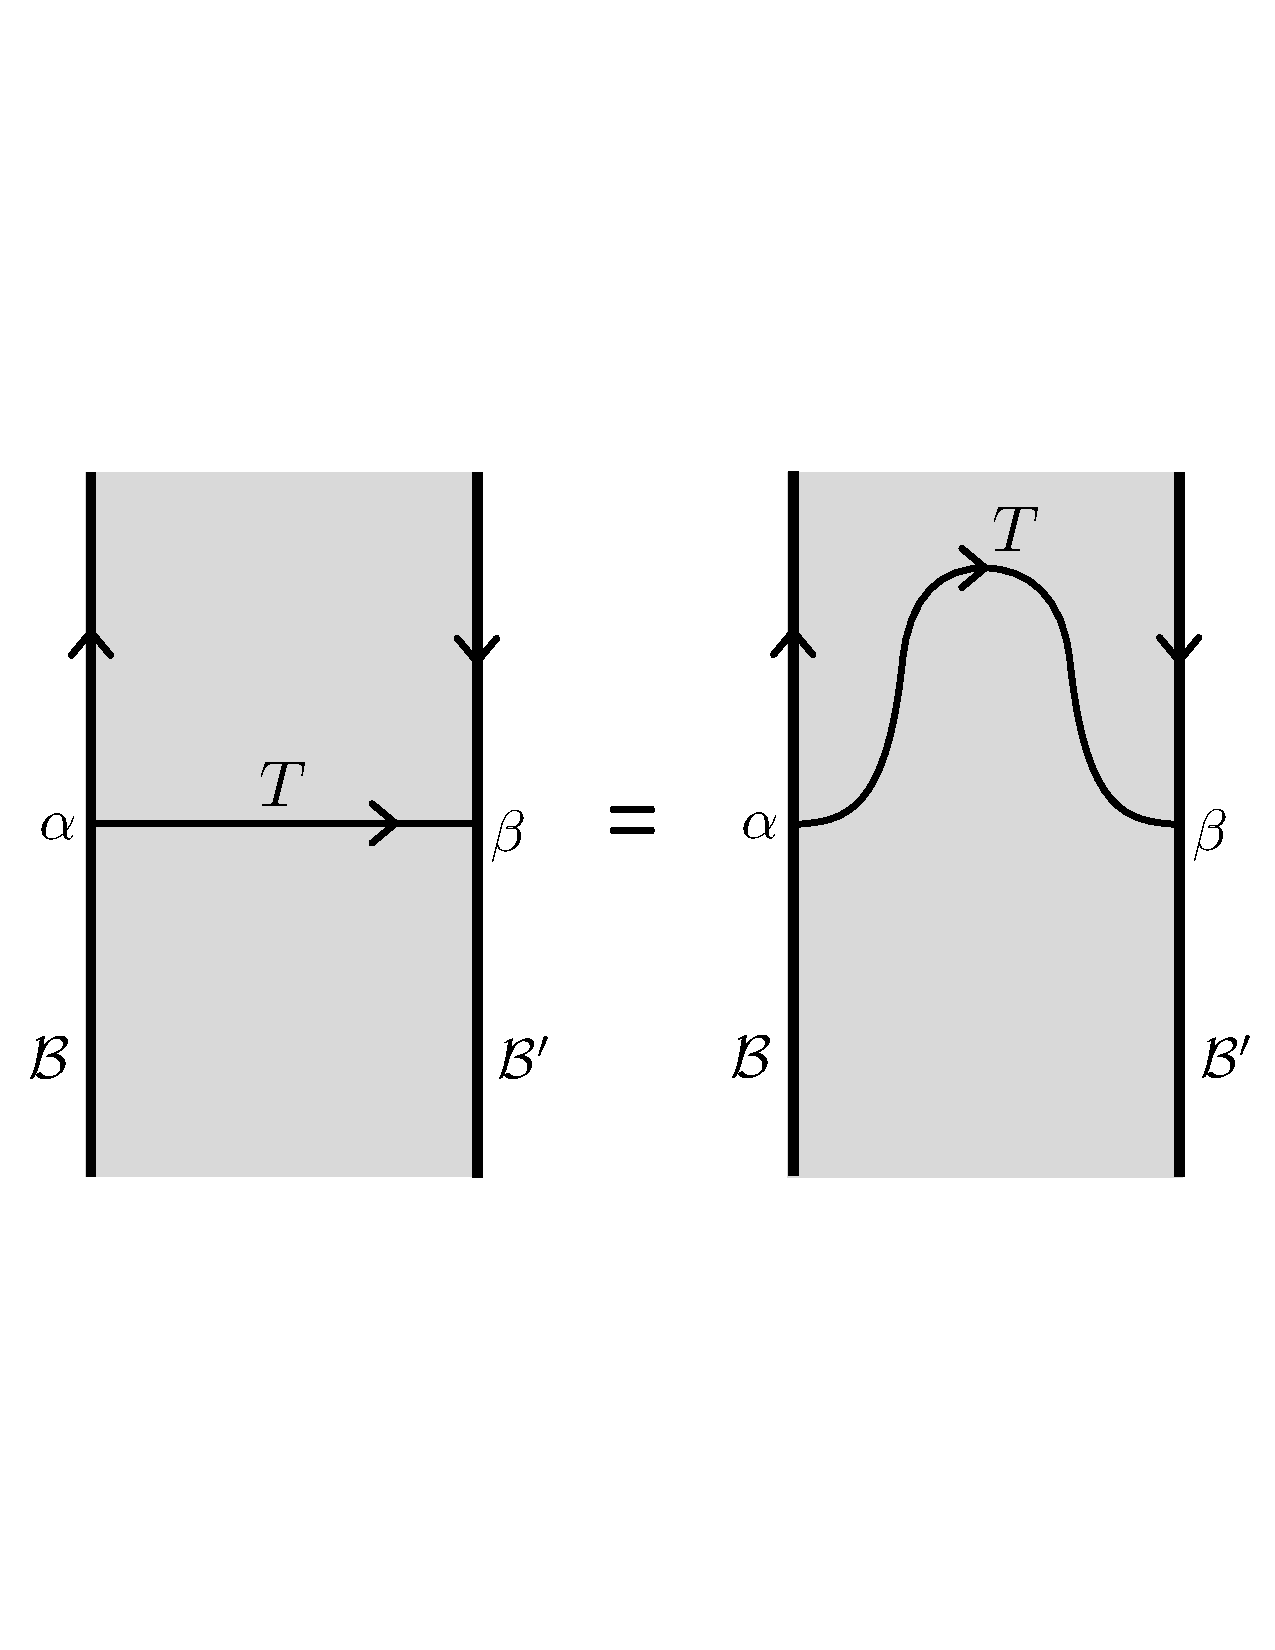
\includegraphics[width=3.4in]{Example2.pdf}
 \end{center}
\caption{\small 本图说明正文中所述的一个代数操作。从下往上读右图，先遇到的是图 \ref{example1}(c,d) 所勾勒的运算，随后是把线算符的乘积 $T'T$ 融合为“恒等”，即融合为平凡线算符。 \label{example2}}
\end{figure} 




在几何朗兰兹对偶的解析进路中 \cite{EFK,EFK2}，Hecke 算符成为作用在量子态希尔伯特空间上的普通算符，而不再是作用在范畴上的更抽象的函子。不出所料，这种意义上的 Hecke 算符的规范场论解释，依据的仍是与前面相同的 't Hooft 线算符，只是用法略有不同。在图 \ref{example1}(b) 中，我们考虑与前面相同的线算符，只不过它现在从图的左侧延伸到右侧。在线算符终止于条带边界的左右两个端点处，必须补充某些额外数据。\zy{译者按（无外部依据）：原文的 strip 指图中画成条带的二维流形 $\Sigma$，其左右两条边界即 $\Sigma$ 的两条边界分支；线算符横穿条带时两端分别落在其上。译文统一作“条带”。}我们暂且假定这些数据已经给定。于是该线算符就成为作用在量子态上的普通算符。从下往上读这幅图：一个 $\Hom(\B',\B)$ 中的元素从底部进入，经过线算符的作用之后，从顶部出来的是一个（可能不同的）$\Hom(\B',\B)$ 中的元素。（若从上往下读，则看到转置算符作用在对偶向量空间 $\Hom(\B,\B')$ 上。）正因为支撑在固定时刻空间中的一维流形上的线算符能够以这种方式充当普通的量子算符，它们传统上\footnote{在粒子物理的传统应用中，没有边界，线算符的支撑集取为闭合回路。此时该算符常被称为圈算符（loop operator）。}才被称为线“算符”。



图 \ref{example1}(c,d) 的目的是解释图 \ref{example1}(b) 中的线算符在左边界或右边界终止处究竟发生了什么。在图 \ref{example1}(c) 中我们看到，线算符的左端点对应一个元素 $\alpha\in\Hom(\B,T\B)$；在图 \ref{example1}(d) 中我们看到，右端点对应一个元素 $\beta\in \Hom(T\B',\B')$。在代数上，带有额外数据 $\alpha,\beta$ 的线算符 $T$ 所对应的算符 $\h T:\Hom(\B',\B)\to \Hom(\B',\B)$ 可以描述如下。对 $\psi\in \Hom(\B',\B)$，有 $\alpha\circ\psi\circ\beta\in \Hom(T\B',T\B)=\Hom(\B',T'T\B)$。再利用线算符构成一个代数、且平凡线算符出现在乘积 $T'T$ 中这两点，便得到映射 $w:\Hom(\B',T'T\B)\to \Hom(\B' ,\B)$。最后，$\h T(\psi)=w\circ\alpha\circ\psi\circ\beta$。这一连串代数操作对应图 \ref{example2} 的画面。对于由线算符 $T$ 或 $T_{R,p}$ 连同端点数据 $\alpha,\beta$ 构造出的 $\H$ 上的算符，我们有时将其记作 $\h T_{\alpha,\beta}$ 或 $\h T_{R,p,\alpha,\beta}$。

\begin{yizhu}[译者按：函子与算符两种图像]
本节的论证可以概括为两个层次的对照。在 Beilinson--Drinfeld 的表述中 \cite{BD}，Hecke 函子作用在 $D$-模或凝聚层的范畴上；在规范场论图像中 \cite{KW}，它对应作用在 $A$-膜范畴上的函子，并由 't Hooft 线算符具体实现。到了 EFK 的解析版本 \cite{EFK,EFK2}，同一个线算符不再是沿边界铺设，而是横穿条带，并在左右两端接上角数据 $\alpha,\beta$，于是成为作用在量子态希尔伯特空间上的普通算符（图 \ref{example1}(b)）。两种图像并不矛盾：把线算符移到边界上便得到函子（图 \ref{example1}(a)），把它的两端接到左右边界上便得到算符；式 $\h T(\psi)=w\circ\alpha\circ\psi\circ\beta$ 正是这一转换的代数表达。
\end{yizhu}


 \begin{figure}
 \begin{center}
   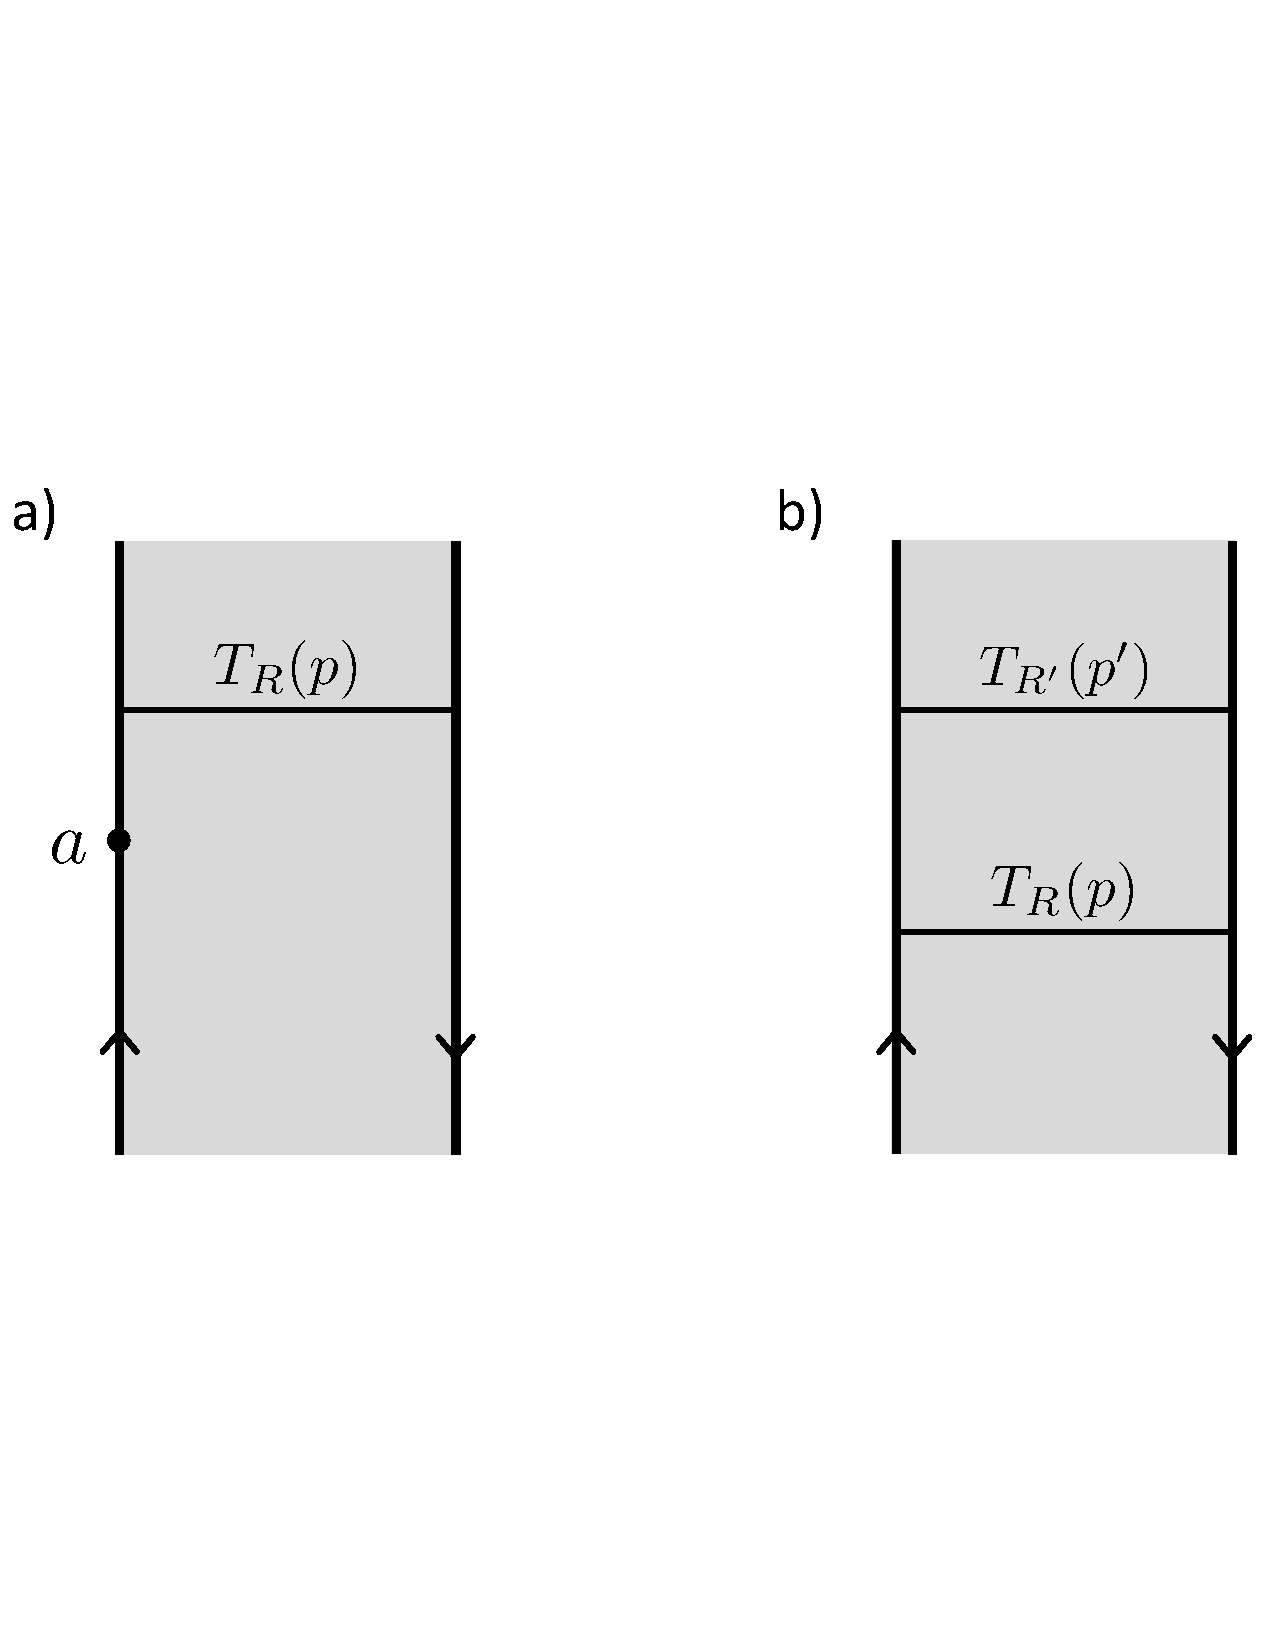
\includegraphics[width=3.4in]{Example3.pdf}
 \end{center}
\caption{\small 证明量子化 Hitchin 哈密顿量彼此交换的论证，可以稍作改动，用来证明线算符（视为量子态空间上的实际算符）与量子化 Hitchin 哈密顿量交换，并且彼此交换。在两种情形下（分别如 (a) 与 (b) 所示），关键都在于：由于额外维度的存在，两个算符可以毫无奇异地互相上下滑过。 \label{example3}}
\end{figure} 


 \begin{figure}
 \begin{center}
   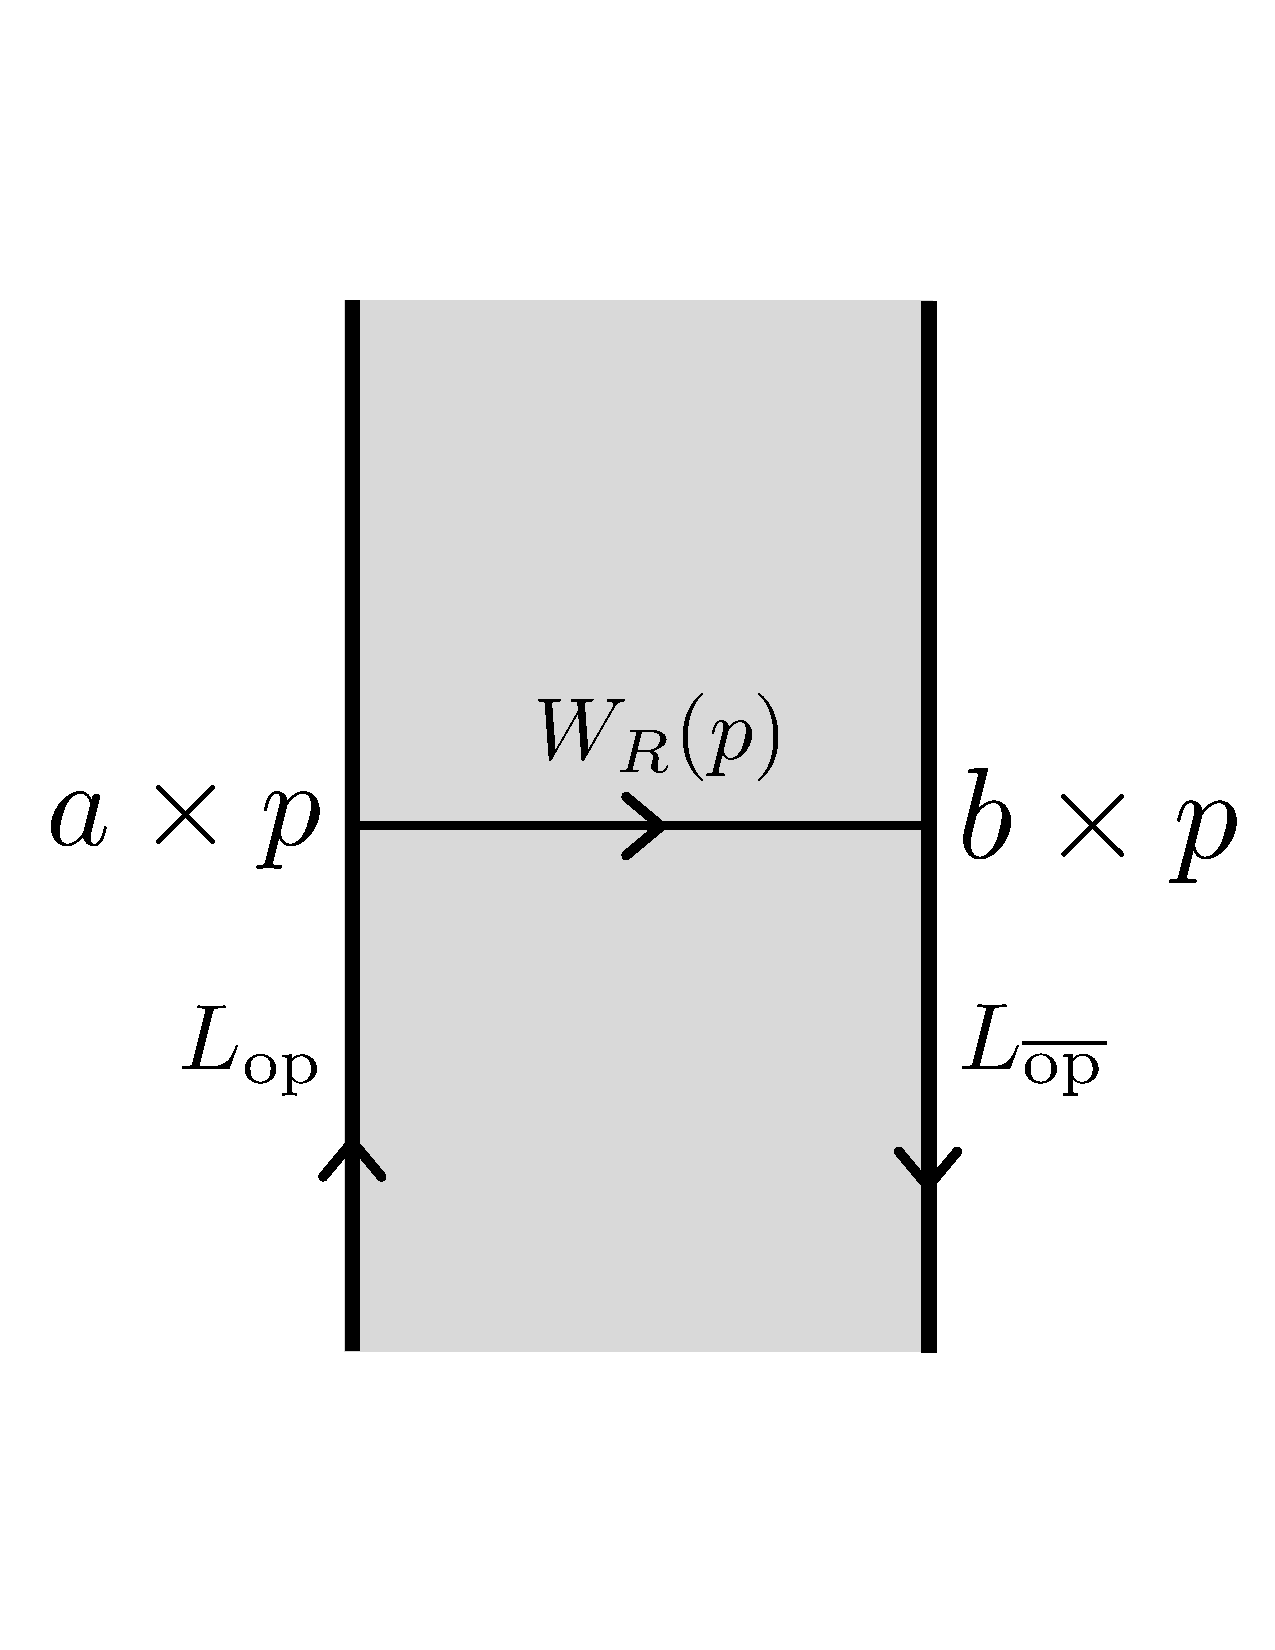
\includegraphics[width=2.1in]{Example4b.pdf}
 \end{center}
\caption{\small 为计算 't Hooft/Hecke 算符的本征值，人们考虑描述从 $a\times p$ 到 $b\times p$ 的平行移动的对偶 Wilson 算符，其中 $p$ 是 $C$ 中的一点，$a,b$ 是 $\Sigma$ 左右边界上的点。 \label{example4}}
\end{figure} 

我们将特别关注这样的元素 $(\alpha,\beta)$：它们起源于四维线缺陷落在四维边界条件上的局部端点，而这些四维边界条件分别是 $\B$ 与 $\B'$ 的提升。正如第 \ref{background} 节所言，我们所考虑的边界条件的四维提升不是拓扑的；它们分别是全纯-拓扑的与反全纯-拓扑的。因此，对应于 $\alpha$ 的局部端点将全纯地依赖 $p$，而对应于 $\beta$ 的局部端点将反全纯地依赖 $p$。注意，线缺陷在四维中的实际路径无关紧要，只要它在拓扑上等价于一条笔直路径即可。真正重要的只是端点在 $C$ 中的位置。

't Hooft 算符或 Hecke 算符（如 \cite{EFK,EFK2} 那样视为量子态上的算符）的主要性质之一是：它们彼此交换，并且与量子化 Hitchin 哈密顿量交换。这可由我们先前用来证明 Hitchin 哈密顿量彼此交换的同一推理得到。't Hooft 算符 $T_{R,p}$ 与 Hitchin 哈密顿量 $H_{\P,\alpha}$ 交换，因为可以假定 $\alpha$ 的支撑集与点 $p$ 不相交，从而让 $T_{R,p}$ 与 $H_{\P,\alpha}$ 毫无奇异地互相上下滑过（图 \ref{example3}(a)）。同样，对互不相同的点 $p,p'\in C$，'t Hooft 算符 $T_{R,p}$ 与 $T_{R',p'}$ 交换（图 \ref{example3}(b)）。取极限 $p'\to p$ 便知，即使 $R\not= R'$，$T_{R,p}$ 与 $T_{R',p}$ 也交换。

\subsection{Wilson 算符及其本征值}\label{wilop}

由于 't Hooft 算符与 Hitchin 哈密顿量交换，它们可以在同一组基下对角化，即态基 $\psi_{u,\veps},$ $u\in \Upsilon,$ $\veps\in \T_u$，其中 $\Upsilon=L_\op\cap L_\bop$（第 \ref{inccenter} 节）。事实上，我们可以用电–磁对偶来确定 't Hooft 算符的本征值。't Hooft 算符 $T_{R,p}$ 对偶于 Wilson 算符 $W_{R,p}$，后者由 $G^\vee_\C$ 的同一个表示 $R$ 标记，并支撑在同一点 $p\in C$。't Hooft 算符是“无序”（disorder）算符，其微观定义涉及某种奇异性。\zy{“无序算符”（disorder operator）与 Wilson 算符这类“有序算符”（order operator）相对：它不能只由沿回路的经典和乐给出，而要在支撑附近规定场的奇异性或单值。't Hooft 在讨论夸克禁闭时引入了这种算符，见 G. 't Hooft, ``On the phase transition towards permanent quark confinement,'' \emph{Nucl. Phys.} \textbf{B138} (1978) 1。} Wilson 算符则不同：它在经典层面上用和乐（holonomy）定义，如下所述。在四维流形 $M$ 上相应的规范场论中（对我们而言，$M=\Sigma\times C$），有一个带联络 $\cA=A+\i \phi$ 的 $G^\vee_\C$ 丛 $E^\vee_\C\to M$，我们可以给它联系一个向量丛 $E^\vee_R=E^\vee_\C\times_{G^\vee_\C} R$。该丛上的诱导联络仍简记为 $\cA$。Wilson 算符由联络 $\cA$ 在 $E^\vee_R$ 上的和乐构造，一般沿某条带定向的路径 $\gamma\subset M$ 积分。若 $\gamma$ 是闭合回路，则取绕 $\gamma$ 的和乐的迹，这样就得到一个在许多物理应用中很重要的 Wilson 算符版本。

然而，要计算由横跨条带的 't Hooft 线算符（图 \ref{example1}(b)）所定义的算符的本征值，我们需要考虑同样横跨条带的对偶 Wilson 算符（图 \ref{example4}）。这个 Wilson 算符不是支撑在闭合回路上，而是支撑在一条路径 $\gamma\subset \Sigma\times p$ 上，该路径从条带左边界上的 $a\times p$ 延伸到右边界上的 $b\times p$。

此时，和乐最好理解为从 $a\times p$ 处的纤维 $E^\vee_R$ 到该丛在 $b\times b$ 处的纤维的线性变换。\zy{译者按（无外部依据）：原文此处作 $b\times b$，据上下文及下一式 (\ref{lintr})，应为 $b\times p$；这是原文笔误，译文照录并在此说明。}于是，按这些纤维的显然记号，$W_{R,p}$ 是一个线性变换
\be\label{lintr} W_{R,p}:E^\vee_{R,a\times p}\to E^\vee_{R, b\times p}.\ee
为了更对称地处理条带的左右两边缘，方便的做法是引入与 $R$ 对偶的表示 $R'$，并把 $W_{R,p}$ 视为某个表示上的线性函数。于是有
\be\label{bintr} W_{R,p}\in \Hom(E^\vee_{R,a\times p}\otimes E^\vee_{R',b\times p},\C). \ee

至此，我们得到的是向量空间上的一个线性函数，而不是联络的复值函数；只有后者才能量子化而得到量子算符。要得到联络的复值函数，我们需要给出向量 $v\in E^\vee_{R,a\times p}$、$w\in E^\vee_{R',b\times p}$。此时 $W_{R,p}(v\otimes w)$ 就是一个复值函数，可以量子化而得到算符。

第 \ref{localoper} 节描述了构造合适向量的一种自然方式。在式 (\ref{linmap}) 中，我们对带有伴丛 $E^\vee_R$ 的全纯 oper 描述了一个“最高权截面” $s_R:K_C^{(N-1)/2}\to E^\vee_R$。因此，若给定向量 $v\in K_{C,p}^{(N-1)/2}$，便可定义 $s_R(v)\in E^\vee_{R,p}$。类似地，若 $E^\vee_{R'}$ 是反全纯 oper，则有 $\bar s_{R'}:\bar K_C^{(N-1)/2}\to E^\vee_{R'}$，从而对 $w\in K_{C,p}^{(N-1)/2}$，有 $\bar s_{R'}(w)\in E^\vee_{R',p}$。注意，对偶的表示对 $R,R'$ 具有相同的 $N$ 值。

若丛 $E^\vee_R\to \Sigma\times C$ 在左边界上是全纯 oper、在右边界上是反全纯 oper，我们就可以在左边界上应用这一构造的全纯版本、在右边界上应用其反全纯版本，从而得到
\be\label{wintr}W_{R,p,v\otimes w}=W_{R,p}(s_{R}(v)\otimes \bar s_{R'}(w)). \ee
这最终是联络的一个复值函数，可以量子化而得到物理态上的 Wilson 算符。我们把这个算符称为 $W_{R,p,v\otimes w}$。在这一记号中，我们利用了如下事实：式 (\ref{wintr}) 的右端只通过组合 $v\otimes w$ 依赖于 $v$ 与 $w$。我们用同一记号表示经典和乐（或其矩阵元）与相应的量子算符，希望这不会造成严重混淆。

由于 $B$-模型局域化在平坦联络上，这个算符的对角化是平凡的。\zy{局域化（localization）指拓扑扭化理论的路径积分只由满足经典运动方程的特殊构型贡献。二维 $B$-模型依赖于靶空间的复结构，其路径积分局域化在常数映射上（E. Witten, ``Mirror manifolds and topological field theory,'' in \emph{Essays on Mirror Manifolds}, 1992; arXiv:hep-th/9112056）；在本文中，这些常数映射对应 $C$ 上的平坦联络。}满足边界条件、在边界上取定中心部分的平凡化、并模去规范变换的平坦联络，与使 Hitchin 哈密顿量对角化的通常态基 $\psi_{u,\varepsilon}$（$u\in\Upsilon,$ $\varepsilon\in \T_u$）一一对应。Wilson 算符在这组基下是对角的。量子算符 $ W_{R,p,v\otimes w}$ 在给定基向量 $\psi_{u,\varepsilon}$ 上的本征值，正是相应的经典函数在与 $\psi_{u,\varepsilon}$ 对应的经典解上的取值。这个值就是向量 $s_{R}(v)$ 与 $\bar s_{R'}(w)$ 在对偶向量空间 $E^\vee_{R,p}$ 与 $E^\vee_{R',p}$ 中的自然对偶配对 $(s_R(v), \bar s_{R'}(w))$。之所以如此，是因为 $\Sigma\times C$ 上的平坦联络实际上是从 $C$ 拉回的。

中心 $\zZ(G^\vee)$ 通过 $(s_\ell, s_r)\to (b s_\ell, s_r)$ 作用在物理希尔伯特空间 $\H$ 上（第 \ref{opergauge} 节）。这会把 $\h W_{R,p}$ 的本征值乘上一个单位根，而这个单位根正是中心元素 $b$ 在表示 $R$ 中的值。例如，若 $G^\vee=\SL(n,\C)$ 且 $R$ 是 $n$ 维表示，则 $\h W_{R,p}$ 的本征向量以 $n$ 元组的形式出现，形如 $\lambda\exp(2\pi \i k/n)$，$\lambda\in\C$，$k=0,1,\cdots, n-1$。这与下述事实相对偶：在 $A$-模型一侧，希格斯丛模空间具有由特征类 $\zeta\in H^2(C,\pi_1(G))$ 标记的若干连通分支。对 $G^\vee=\SL(n,\C)$，共有 $n$ 个分支，它们被与 $\h W_{R,p}$ 对偶的 't Hooft 算符 $\h T_{R,p}$ 循环置换，从而导致相同的谱结构。一般地，$\zZ(G^\vee)$ 在 $R$ 上的作用，映照出 $\h T_{R,p}$ 置换模空间各分支的方式。

定义算符 $W_{R,p}$ 所需的全纯与反全纯角数据（corner data），恰恰由向量 $v\in K_C^{(N-1)/2}$、$w\in \bar K_C^{(N-1)/2}$ 构成。对 $\SL(n,\C)$ 的 $n$ 维表示，有 $N=n$。我们预期，为对偶的 't Hooft 算符定义全纯与反全纯角数据也需要同样的数据。


这些可以说是最简单的 Wilson 算符，我们称之为主 Wilson 算符（principal Wilson operator）。然而，若表示 $R$ 限制到 $\g^\vee$ 的主 $\su(2)$ 子代数上时可约，则可以使用更一般的对象 $s_{R,n}:Q_n\otimes K_C^{(n-1)/2}\to E^\vee_R$（式 (\ref{holmap})）。于是，取 $v\in Q_n \otimes K_C^{(n-1)/2}$、$w\in \bar Q_{n'}\otimes K_C^{(n'-1)/2}$（其中 $n$ 与 $n'$ 可以独立选取），便可定义 $W_{R,p,n,n',v\otimes w}=W_{R,p}(s_{R,n}(v)\otimes \bar s_{R',n'}(w))$，它同样可以解释为一个量子力学算符。更一般地，我们还可以考虑 $W_{R,p,n,n',v\otimes w} $ 关于 $p$ 的全纯与反全纯导数。考虑 $n-1$ 个全纯导数与 $n'-1$ 个反全纯导数就足够了；这足以定义一组完备的 Wilson 算符，因为这相当于把线性形式 $W_{R,p}:E^\vee_{R,a\times p}\otimes E^\vee_{R',b\times p}\to \C $（式 (\ref{bintr})）作用到一组向量上，而按第 \ref{localoper} 节的分析，这组向量构成 $W_{R,p}$ 所作用的那个有限维向量空间的一组基。

如果继续求导会怎样？取 $n$ 个全纯导数或 $n'$ 个反全纯导数，我们就会遇到 Wilson 算符 $W_{R,p,n,n',v\otimes w} $ 所满足的微分方程。用来定义这些 Wilson 算符的全纯与反全纯截面 $ s_{R,r}$ 与 $\bar s_{R',n'}$，作为 $p$ 的函数满足某些全纯与反全纯微分方程（第 \ref{localoper} 节与附录 \ref{somex}），相应的 Wilson 算符也满足同样的方程。


在定义了作用在物理希尔伯特空间 $\H$ 上的算符之后，自然要问它们满足什么代数。在体空间（bulk）中，线算符的乘积模拟 $G^\vee $ 的表示的张量积。因此，若 $R_i\otimes R_j\cong \oplus_k N^k_{ij}R_k$，其中 $N^k_{ij}$ 是向量空间，则相应的平行 Wilson 算符的分解为 $W_{R_i} W_{R_j}=\oplus_k N^k_{ij} W_k$。对于把 Wilson 算符理解为作用在边界条件上的函子这一观点，这正是恰当的关系，如图 \ref{example1}(a) 所示。原则上，由这一代数可以重构非阿贝尔群 $G^\vee $ 的结构。然而，对于此处所讨论的把 Wilson 算符作为量子态上的算符这一观点，情况有所不同。若相乘的是两个主 Wilson 算符——它们与相应表示中的最高权向量相联系——情形最为简单。由于两个表示 $R_1$ 与 $R_2$ 中最高权向量的张量积是张量积 $R_1\otimes R_2$ 中的最高权向量，两个主 Wilson 线算符的乘积仍是主 Wilson 线算符，对应于一个表示 $R_3$，其最高权是 $R_1$ 与 $R_2$ 的最高权之和。若相乘更一般的 Wilson 算符 $W_{R,p,n,n',v\otimes w}$ 及其导数，我们就会看到非阿贝尔群的结构。

用 $S$-对偶数据定义的对偶 't Hooft 算符，自然具有与 Wilson 算符相同的本征值。主要的困难在于精确辨识出适当的 $A$-模型端点。我们将在第 \ref{dualhooft} 节转向这一问题。

我们以如下评述结束关于 Wilson 算符的讨论。在四维规范场论中，oper 边界条件最有启发的实现涉及 Nahm 极点 \cite{GWknots}。与早先假定的较直接进路 \cite{KW}（其中边界条件只通过在边界上指定 $\cA$ 的 $(0,1)$ 或 $(1,0)$ 部分来定义）相比，oper 边界条件的 Nahm 极点描述有两个优点：它直接导致第 \ref{localoper} 节所讨论的局部约束；并且它还为通过 $\B_\cc$ 与 $A$-模型描述的对偶给出了简单的解释。若采用 oper 边界条件的 Nahm 极点描述，则复联络 $\cA$ 沿边界是奇异的，因而在定义横穿条带的经典和乐 $W_R$ 以及相应的量子算符时，需要某种重整化。这种重整化相当于作一个复规范变换，以消去 Nahm 极点奇异性。


   

